\documentclass{standalone}
\usepackage{tikz}
\usepackage{ctex,siunitx}
\usepackage{tkz-euclide}
\usepackage{amsmath}
\usetikzlibrary{patterns, calc}
\usetikzlibrary {decorations.pathmorphing, decorations.pathreplacing, decorations.shapes,}
\begin{document}
\small
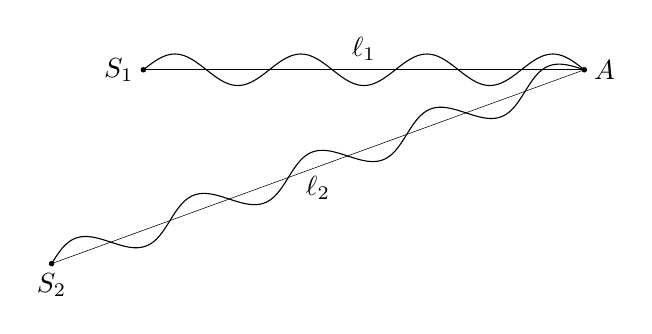
\begin{tikzpicture}[>=stealth, scale=1, samples=200]
  \draw [domain=-5.6:0]  plot (\x,{-0.2*sin(1.25*pi*\x r)});
  \draw [very thin] (0,0)--(-5.6,0)node[midway,above]{$\ell_1$};
  \fill(0,0)circle(1pt)node[right]{$A$};
  \fill(-5.6,0)circle(1pt)node[left]{$S_1$};
  \begin{scope}[rotate=20]
    \draw [domain=-7.2:0]  plot (\x,{-0.2*sin(1.25*pi*\x r)});
    \draw [very thin] (0,0)--(-7.2,0)node[midway,below]{$\ell_2$};
    \fill(-7.2,0)circle(1pt)node[below]{$S_2$};
  \end{scope}
\end{tikzpicture}
\end{document}